\documentclass{standalone}
\usepackage{tikz}
\begin{document}
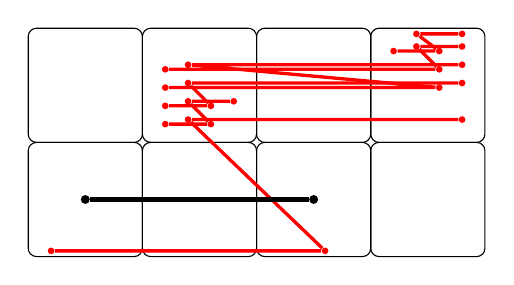
\begin{tikzpicture}[scale=1.45]
  % draw rounded cell boxes
  \draw[rounded corners=3pt] (0,0) rectangle (1,1);
  \draw[rounded corners=3pt] (0,1) rectangle (1,2);
  \draw[rounded corners=3pt] (1,0) rectangle (2,1);
  \draw[rounded corners=3pt] (1,1) rectangle (2,2);
  \draw[rounded corners=3pt] (2,0) rectangle (3,1);
  \draw[rounded corners=3pt] (2,1) rectangle (3,2);
  \draw[rounded corners=3pt] (3,0) rectangle (4,1);
  \draw[rounded corners=3pt] (3,1) rectangle (4,2);
  \node[circle, fill=red, inner sep=0.03cm] (obs4405691552_pt0) at (0.2,0.05) {};
  \node[circle, fill=red, inner sep=0.03cm] (obs4405691552_pt1) at (1.4,1.2) {};
  \node[circle, fill=red, inner sep=0.03cm] (obs4405691552_pt2) at (2.6,0.05) {};
  \node[circle, fill=red, inner sep=0.03cm] (obs4405691552_pt3) at (3.8,1.2) {};
  \draw[red, line width=1.2pt] (obs4405691552_pt0) -- (obs4405691552_pt2) -- (obs4405691552_pt1) -- (obs4405691552_pt3);
  \node[circle, fill=red, inner sep=0.03cm] (obs4405691600_pt0) at (1.2,1.16) {};
  \node[circle, fill=red, inner sep=0.03cm] (obs4405691600_pt1) at (1.4,1.3599999999999999) {};
  \node[circle, fill=red, inner sep=0.03cm] (obs4405691600_pt2) at (1.6,1.16) {};
  \node[circle, fill=red, inner sep=0.03cm] (obs4405691600_pt3) at (1.8,1.3599999999999999) {};
  \draw[red, line width=1.2pt] (obs4405691600_pt0) -- (obs4405691600_pt2) -- (obs4405691600_pt1) -- (obs4405691600_pt3);
  \node[circle, fill=red, inner sep=0.03cm] (obs4405691648_pt0) at (1.2,1.32) {};
  \node[circle, fill=red, inner sep=0.03cm] (obs4405691648_pt1) at (1.4,1.52) {};
  \node[circle, fill=red, inner sep=0.03cm] (obs4405691648_pt2) at (1.6,1.32) {};
  \node[circle, fill=red, inner sep=0.03cm] (obs4405691648_pt3) at (3.8,1.52) {};
  \draw[red, line width=1.2pt] (obs4405691648_pt0) -- (obs4405691648_pt2) -- (obs4405691648_pt1) -- (obs4405691648_pt3);
  \node[circle, fill=red, inner sep=0.03cm] (obs4405691696_pt0) at (1.2,1.48) {};
  \node[circle, fill=red, inner sep=0.03cm] (obs4405691696_pt1) at (1.4,1.68) {};
  \node[circle, fill=red, inner sep=0.03cm] (obs4405691696_pt2) at (3.6,1.48) {};
  \node[circle, fill=red, inner sep=0.03cm] (obs4405691696_pt3) at (3.8,1.68) {};
  \draw[red, line width=1.2pt] (obs4405691696_pt0) -- (obs4405691696_pt2) -- (obs4405691696_pt1) -- (obs4405691696_pt3);
  \node[circle, fill=red, inner sep=0.03cm] (obs4405691744_pt0) at (1.2,1.6400000000000001) {};
  \node[circle, fill=red, inner sep=0.03cm] (obs4405691744_pt1) at (3.4,1.84) {};
  \node[circle, fill=red, inner sep=0.03cm] (obs4405691744_pt2) at (3.6,1.6400000000000001) {};
  \node[circle, fill=red, inner sep=0.03cm] (obs4405691744_pt3) at (3.8,1.84) {};
  \draw[red, line width=1.2pt] (obs4405691744_pt0) -- (obs4405691744_pt2) -- (obs4405691744_pt1) -- (obs4405691744_pt3);
  \node[circle, fill=red, inner sep=0.03cm] (obs4405691792_pt0) at (3.2,1.8) {};
  \node[circle, fill=red, inner sep=0.03cm] (obs4405691792_pt1) at (3.4,1.95) {};
  \node[circle, fill=red, inner sep=0.03cm] (obs4405691792_pt2) at (3.6,1.8) {};
  \node[circle, fill=red, inner sep=0.03cm] (obs4405691792_pt3) at (3.8,1.95) {};
  \draw[red, line width=1.2pt] (obs4405691792_pt0) -- (obs4405691792_pt2) -- (obs4405691792_pt1) -- (obs4405691792_pt3);
  % draw black chords for chord_row_cells
  \node[circle, fill=black, inner sep=0.04cm] (chord_row0_left) at (0.5,0.5) {};
  \node[circle, fill=black, inner sep=0.04cm] (chord_row0_right) at (2.5,0.5) {};
  \draw[black, line width=1.5pt] (chord_row0_left) -- (chord_row0_right);
\end{tikzpicture}
\end{document}